\subsection{Data quality}

In the introduction, we already looked at some key challenges regarding data quality. In this subsection, we will investigate and search solutions for the some of the following typical data quality problems in detail:
\begin{itemize}
  \item \textbf{Incompleteness} - missing instances or attributes
  \item \textbf{Invalidity} - impossible values
  \item \textbf{Inconsitency} - conflicting values
  \item \textbf{Imprecision} - approximates or rounded values
  \item \textbf{Outdated} - values based on old observations
\end{itemize}

For that, we will take a look at missing, invalid, unlikely, and outlier values.

\subsubsection*{Missing values}
Imagine different missing features\sidenote{Missing features} of some instances. Since some data is missing, we need to deal with this in some way. Here are the possible options:
\begin{enumerate}
  \item Remove feature completely (for all instances)
  \item Only consider instsances that have a value (this is done for per-feature-evaluation)
  \item Remove all instances that have one of the features missing
  \item Repair missing features (imputation)
\end{enumerate}

The problem setting and the possible solutions are visualized in \ref{fig:2_missing_values}.

\begin{figure}[h]
  \centering
  \begin{subfigure}{0.4\textwidth}
    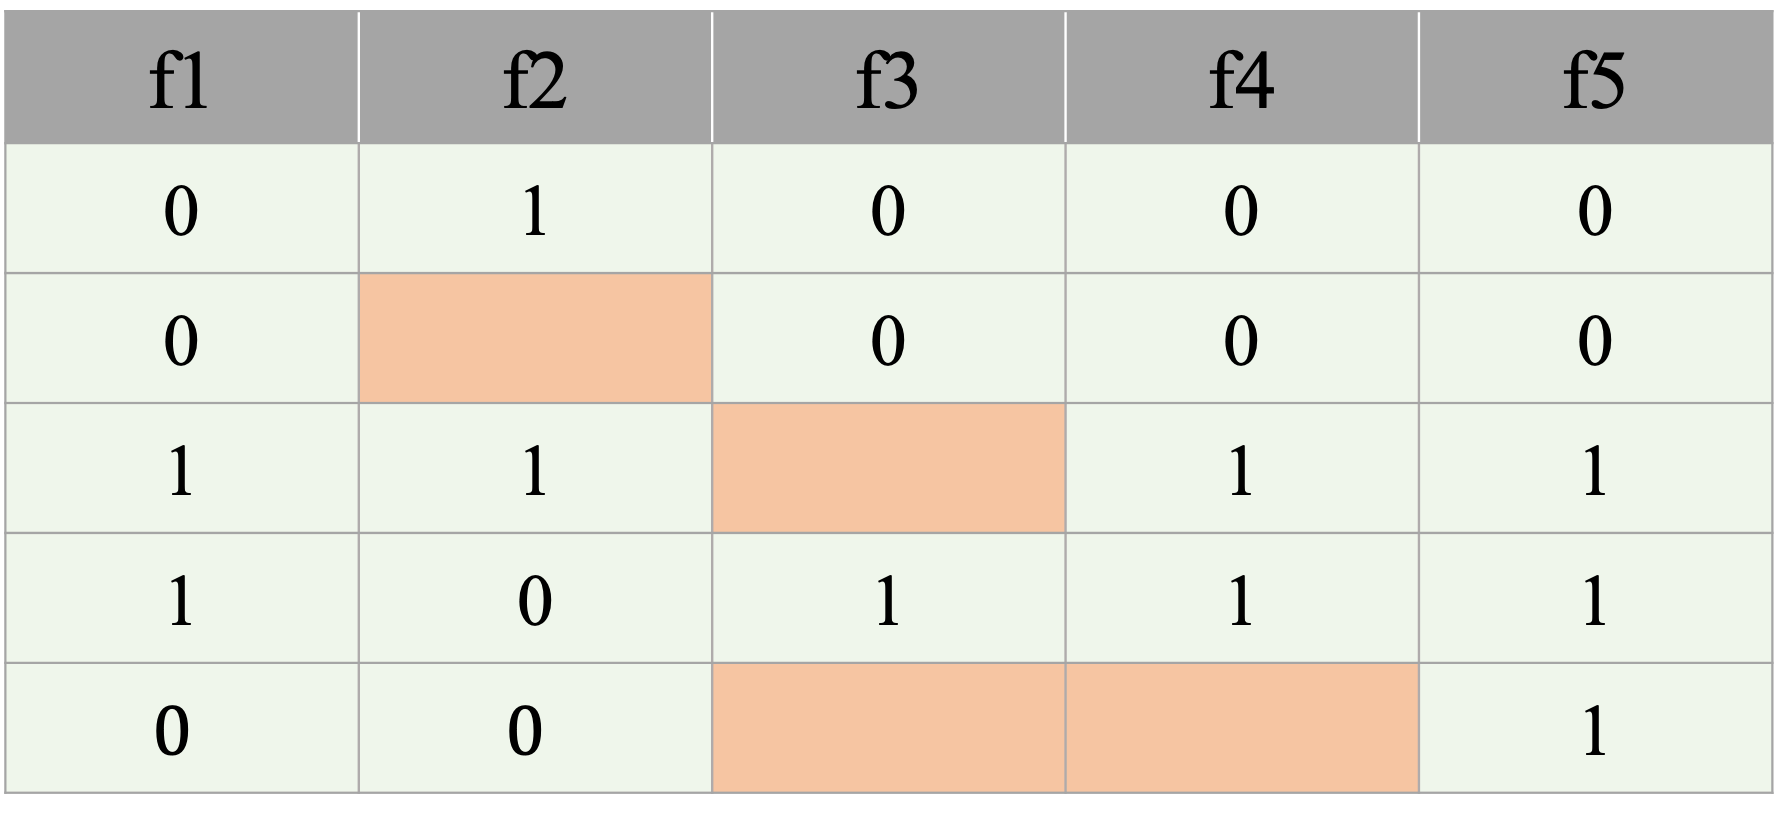
\includegraphics[width=\linewidth]{assets/visualization_and_extraction/problem_missing_values.png}
    \caption{Problem setting}
  \end{subfigure}\\
  \vspace*{0.5cm}
  \begin{subfigure}{0.7\textwidth}
    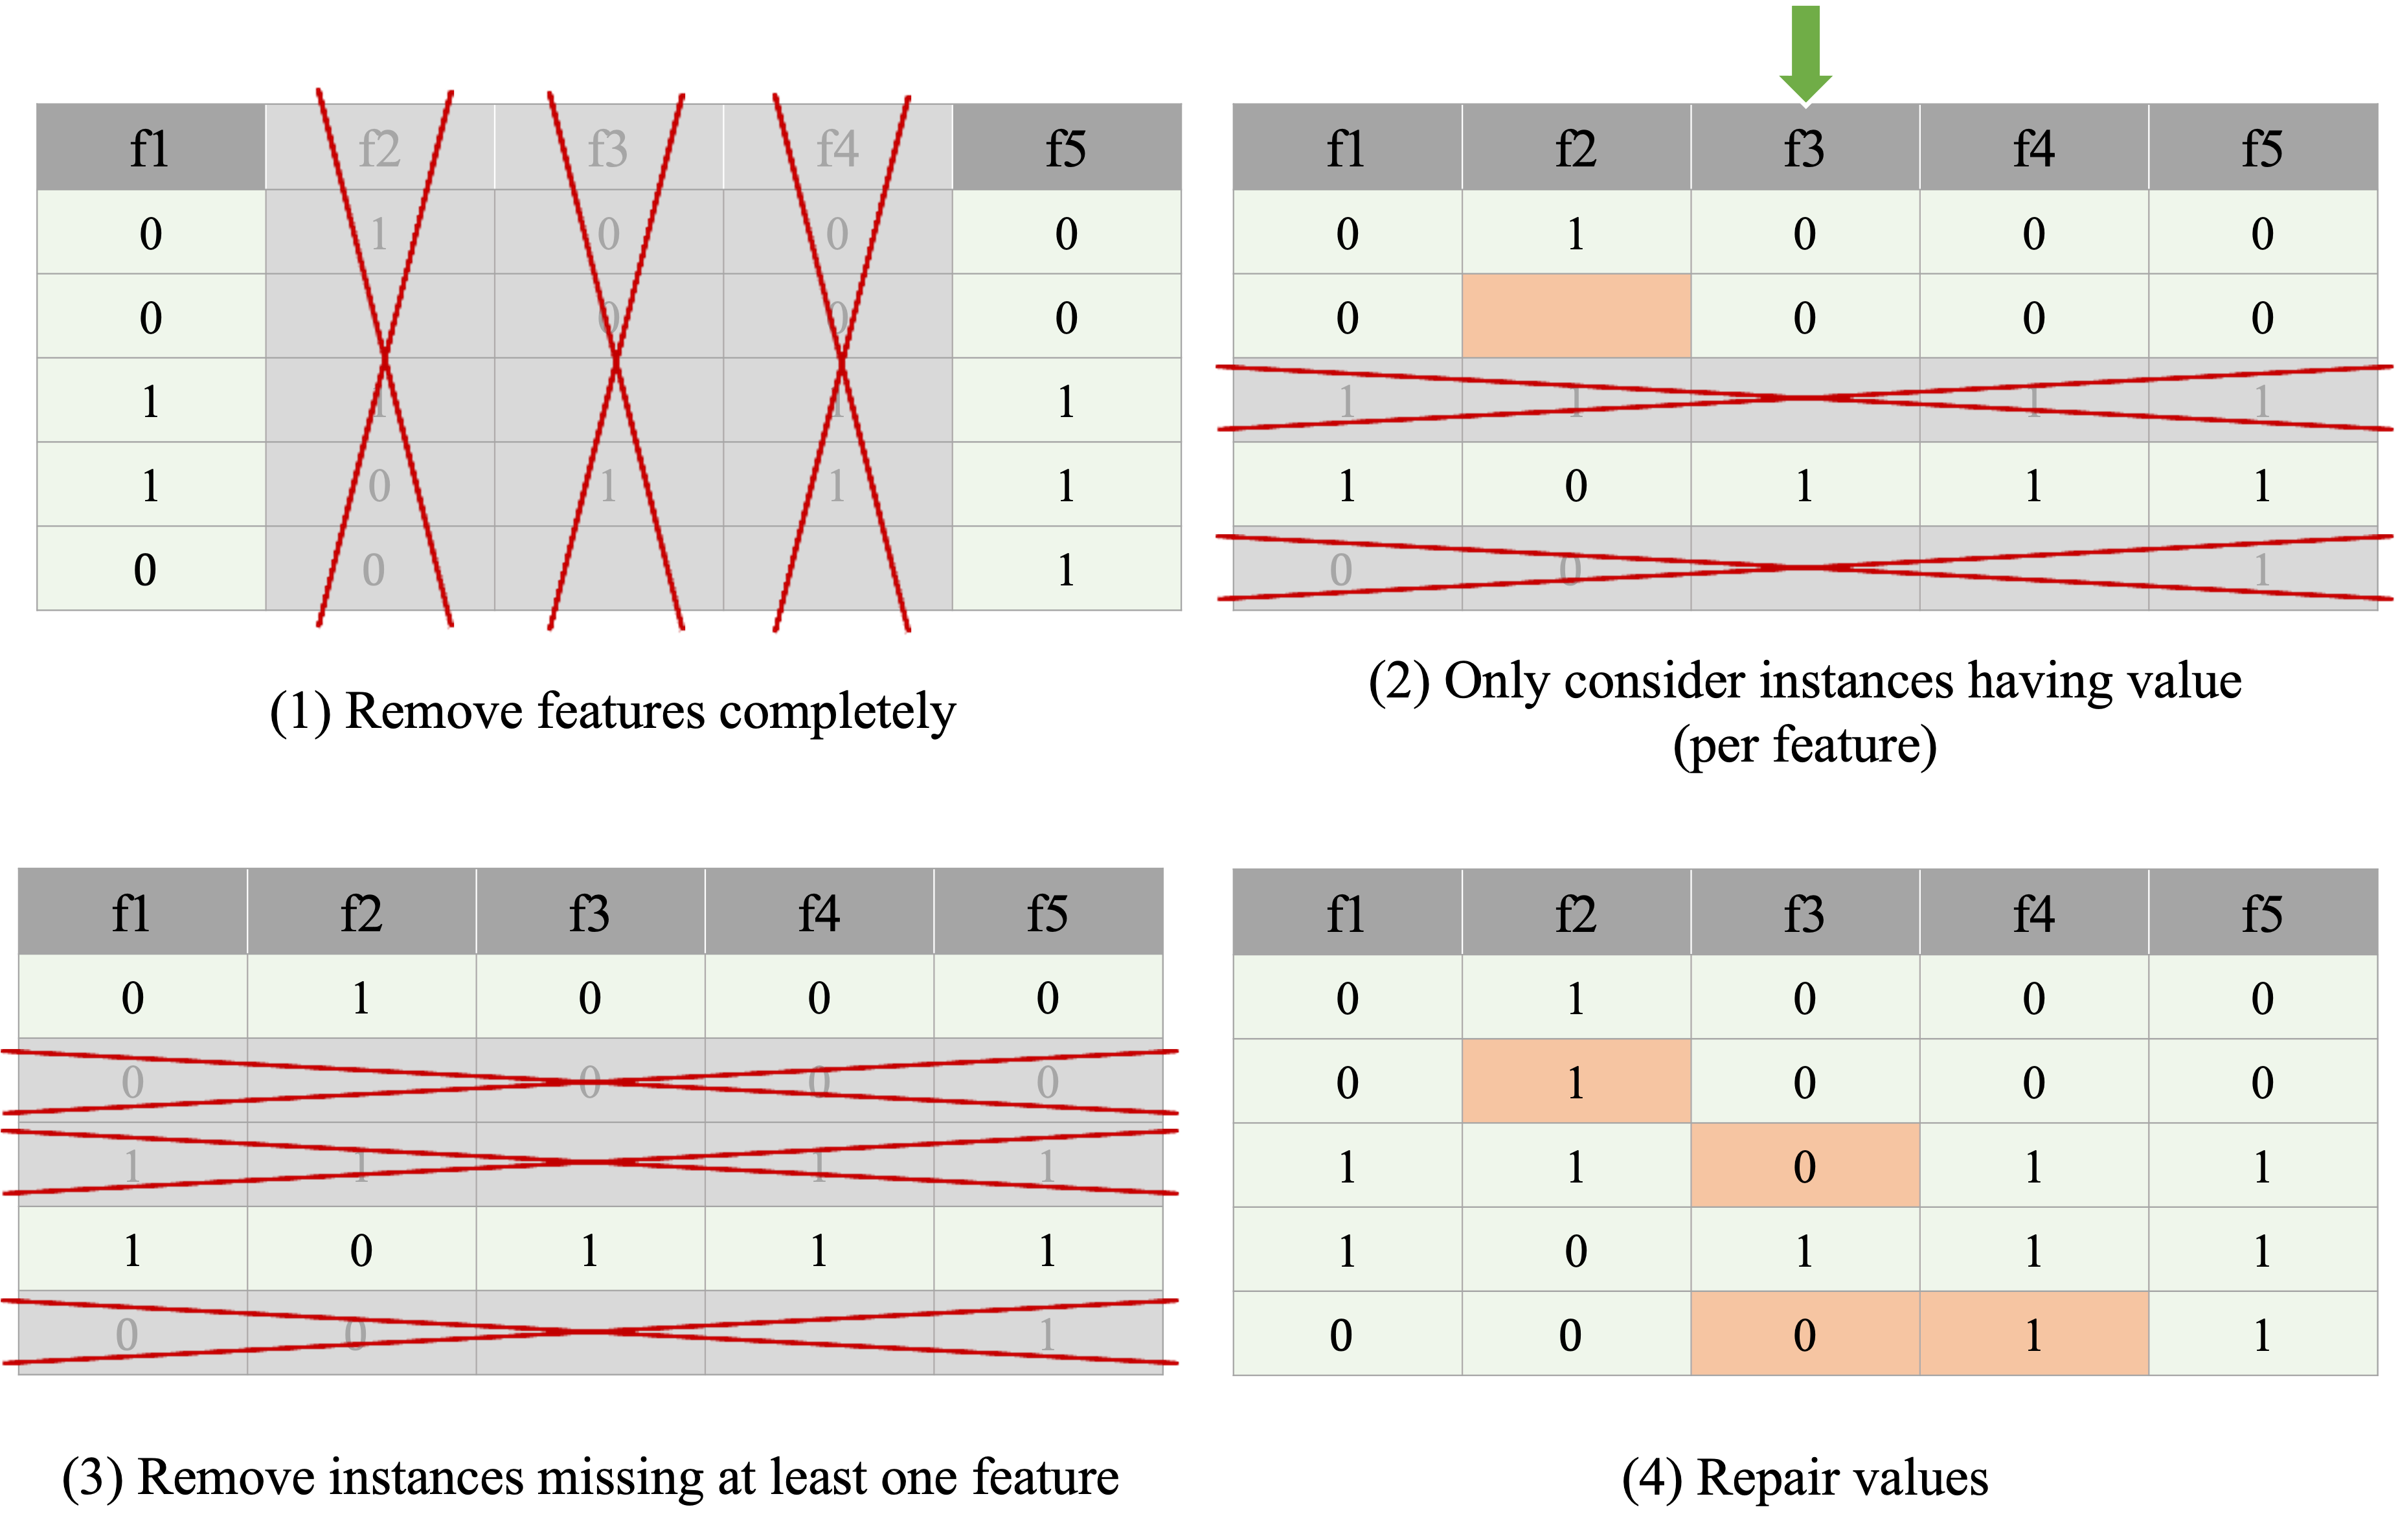
\includegraphics[width=\linewidth]{assets/visualization_and_extraction/solution_missing_values.png}
    \caption{Possible solutions}
  \end{subfigure}
  \caption{Missing values}
  \label{fig:2_missing_values}
\end{figure}

\subsubsection*{Impossible values}
The next typical challenge are impossible values\sidenote{Impossible values} that by some mistake were entered as data. Examples are:
\begin{itemize}
  \item Wrong date format: instead of \textcolor{mathblue}{2018-10-18}, we would have \textcolor{mathblue}{18-10-2018}
  \item Completely impossible date or time: \textcolor{mathblue}{2018-13-51}, \textcolor{mathblue}{23:61}
  \item There can be spelling errors, for example for colors: \textcolor{mathblue}{Bllue}
  \item The data type might not make sense with the feature, like number of members as a float: \textcolor{mathblue}{6.5 member}
\end{itemize}

The handling of this problem is solved just as for missing features.

\subsubsection*{Unlikely values}
In contrast to impossible values, unlikely values are theoretically possible, but just not common to appear. Examples are:
\begin{itemize}
  \item Age: $123$ is rather unlikely, but possible
  \item Price: $120.000\$$ in a store where the other prices lie in the range of $5\$$ to $150\$$
  \item Dates: even on dates, where one would usually expect a uniform distribtion over months and days, days $1$ to $12$ are more frequent than days $13$ to $31$\footnote{NOT the case anymore if date format \textcolor{mathblue}{DD-MM-YYYY} and \textcolor{mathblue}{MM-DD-YYYY} are mixed}
\end{itemize}
Whether a value is unlikely or not is identified based on \textbf{domain knowledge}\sidenote{Unlikely values, domain knowledge}. They can then be further investigated to see, whether the unlikely value is acutally valid.


\subsubsection*{Outlier values}
In contrast to unlikely values, \textbf{outlier values}\sidenote{Outlier values} are identified based on the distribution. 

An especially popular technique to visualize distributions and outliers are \textbf{box plots}\sidenote{Box plot}. They were first introduced by John Tukey in the book "Exploratory data analysis" in 1977. Figure \ref{fig:2_box_plot} shows the properties visualized by a box plot and also how to construct one given a data set. 

\begin{figure}[h]
  \centering
  \subcaptionbox{Properties on a box plot}{
    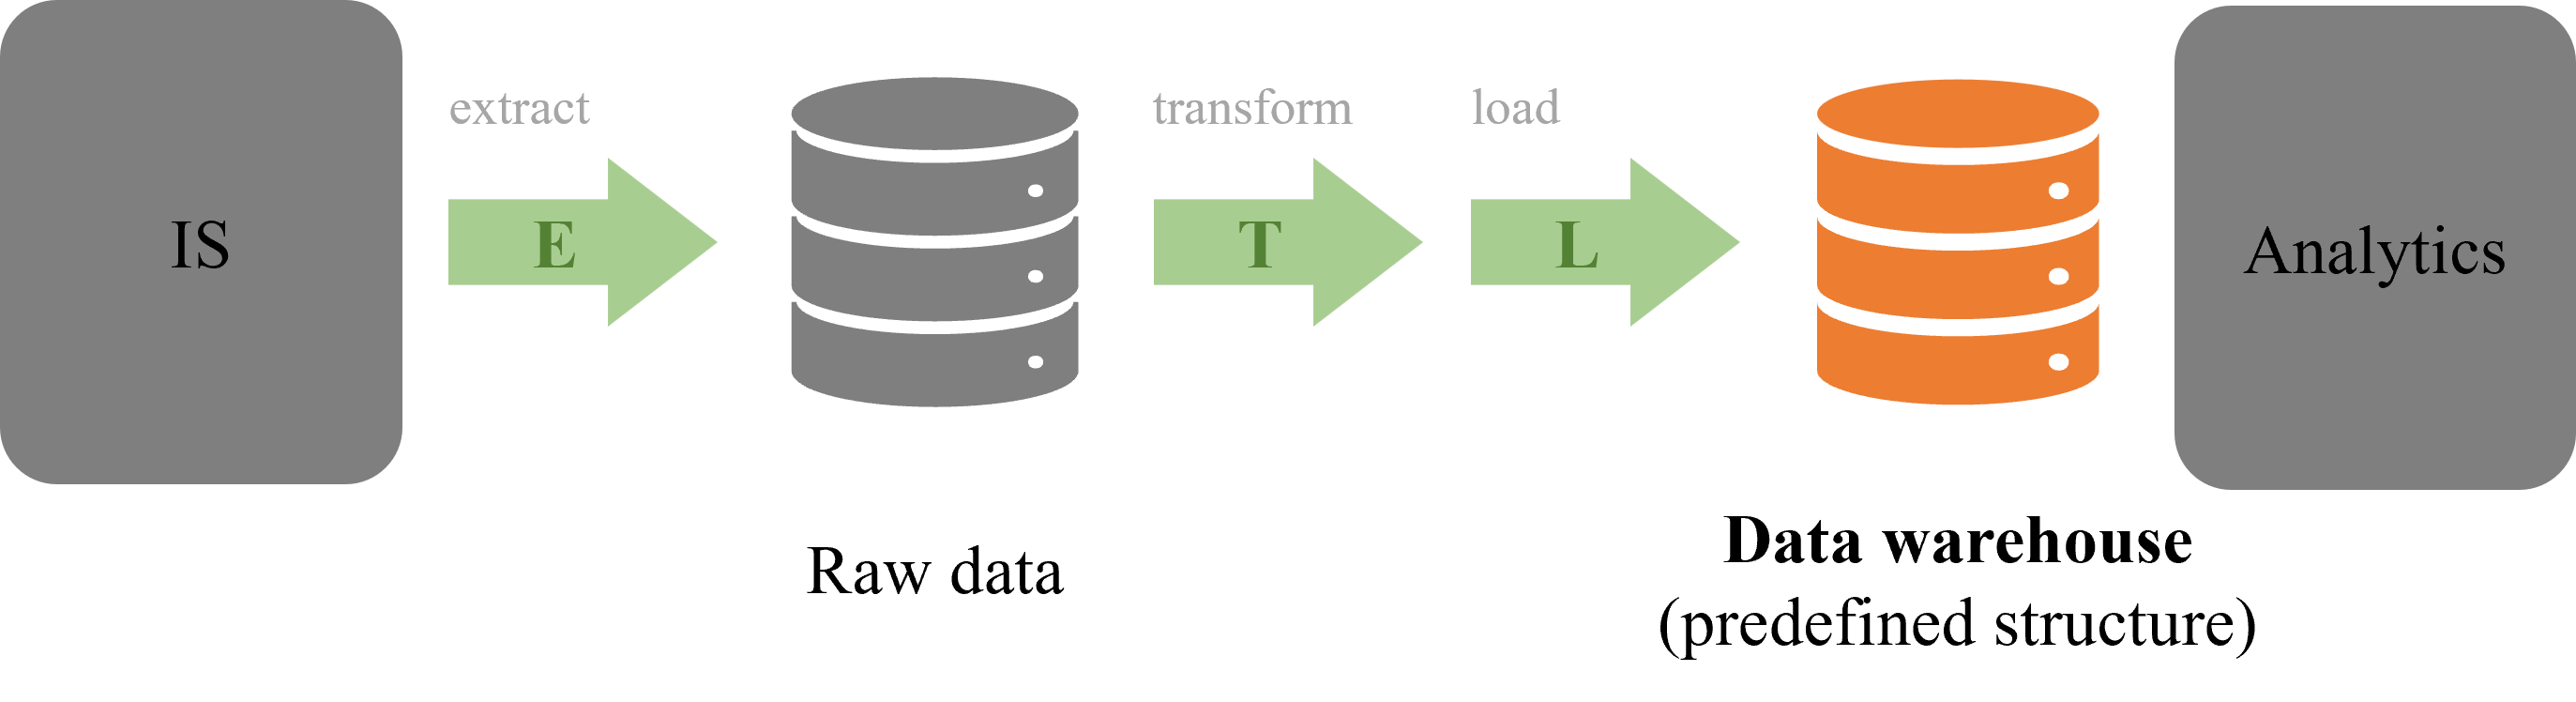
\includegraphics[width=0.45\textwidth]{assets/basics/etl.png}% TODO: adjust
  }
  \hspace*{0.05\textwidth}
  \subcaptionbox{Construction of a box plot}{
    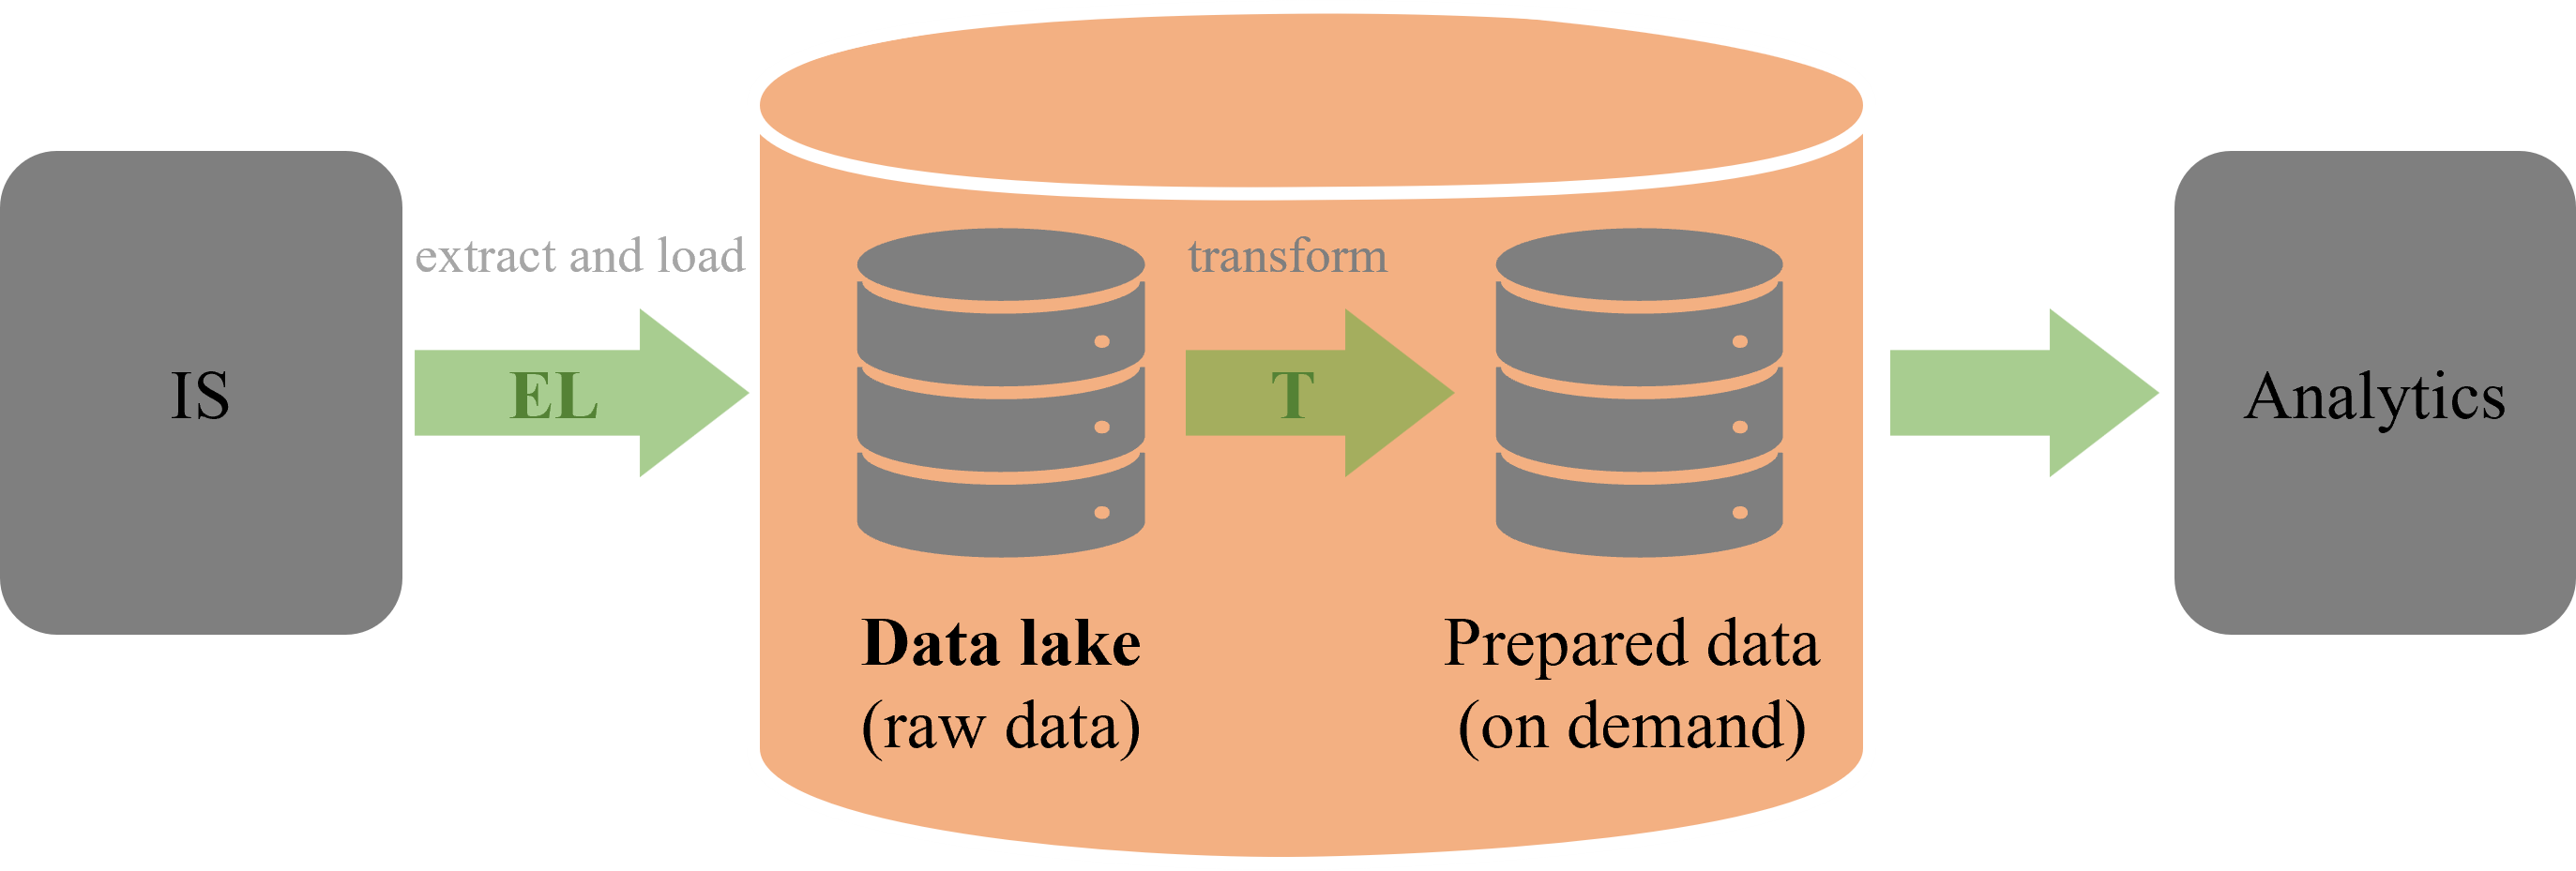
\includegraphics[width=0.45\textwidth]{assets/basics/elt.png}% TODO: adjust
  }
  \caption{Box plot}
  \label{fig:2_box_plot}
\end{figure}

Let's first take a look at the properties one can see in the box diagram. 
\begin{itemize}
  \item The \textbf{median} value\footnote{Median = The "middle" value, so the number halfway between lowest and highest number.} is depicted by the "Bar" in the center.\
  \item The \textbf{IQR}\sidenote{IQR}, so the interquartile range\footnote{First to third quartile, where the first quartile is the number halfway between lowest and middle number, and third quatile is the number halway between middle and highest number.}, covering $50\%$ of the "middle instances" is depicted by the "Box".
  \item The upper whisker indicates the \textbf{maximal} value below the $3^{\text{\color{mathblue}rd}} \text{\color{mathblue} quartile} + 1.5\cdot IQR$, whereas
  \item The lower whisker indicates the \textbf{minimal} value above the $1^{\text{\color{mathblue}st}} \text{\color{mathblue} quartile} - 1.5\cdot IQR$.
  \item Finally, the \textbf{outliers} are drawn separately.
\end{itemize}

The description already contained a bit of the construction details, which will now be explained in more detail with an example. Consider the (already ordered) data set \textcolor{mathblue}{\{ {\tiny \color{gray} 1: }1, {\tiny \color{gray} 2: }2, {\tiny \color{gray} 3: }5, {\tiny \color{gray} 4: }7, {\tiny \color{gray} 5: }8, {\tiny \color{gray} 6: }8, {\tiny \color{gray} 7: }9, {\tiny \color{gray} 8: }9, {\tiny \color{gray} 9: }9, {\tiny \color{gray} 10: }10, {\tiny \color{gray} 11: }10, {\tiny \color{gray} 12: }10, {\tiny \color{gray} 13: }11, {\tiny \color{gray} 14: }12, {\tiny \color{gray} 15: }14, {\tiny \color{gray} 16: }19, {\tiny \color{gray} 17: }23 \}}. Then we construct the box diagram like this:
\begin{itemize}
  \item The median value is $9$ \textcolor{gray}{\tiny(at position 9)}.
  \item The first quatile has the value $8$ \textcolor{gray}{\tiny(at position 5)}, the third one has the value $11$ \textcolor{gray}{\tiny(at position 13)} resulting in an $IQR = 11-8 = 3$.
  \item This means we have an upper fence $11 + 1.5\cdot3 = 15.5$, and the upper whisker as the maximum value below this fence at $14$ \textcolor{gray}{\tiny(position 15)}.
  \item The lower fence has the value $8 - 1.5\cdot3 = 3.5$, the lower whisker therefore the minimum value above this fence value at $5$ \textcolor{gray}{\tiny(position 3)}.
  \item Finally, the outliers are $1, 2, 19, 23$ \textcolor{gray}{\tiny(position 1, 2, 16, 17)}.
\end{itemize}
Those are all the necessary components to construct the box diagram.

Now, one final detail about box diagrams and also the topic of this paragraph is the handling of the outliers. They can first be removed (meaning remove values above and below the upper and lower fences), and their existance can be indicated by claming the removed values to these thresholds. The process is shown in \ref{fig:2_box_plot_outlier_handling}.

\begin{figure}[h]
  \centering
  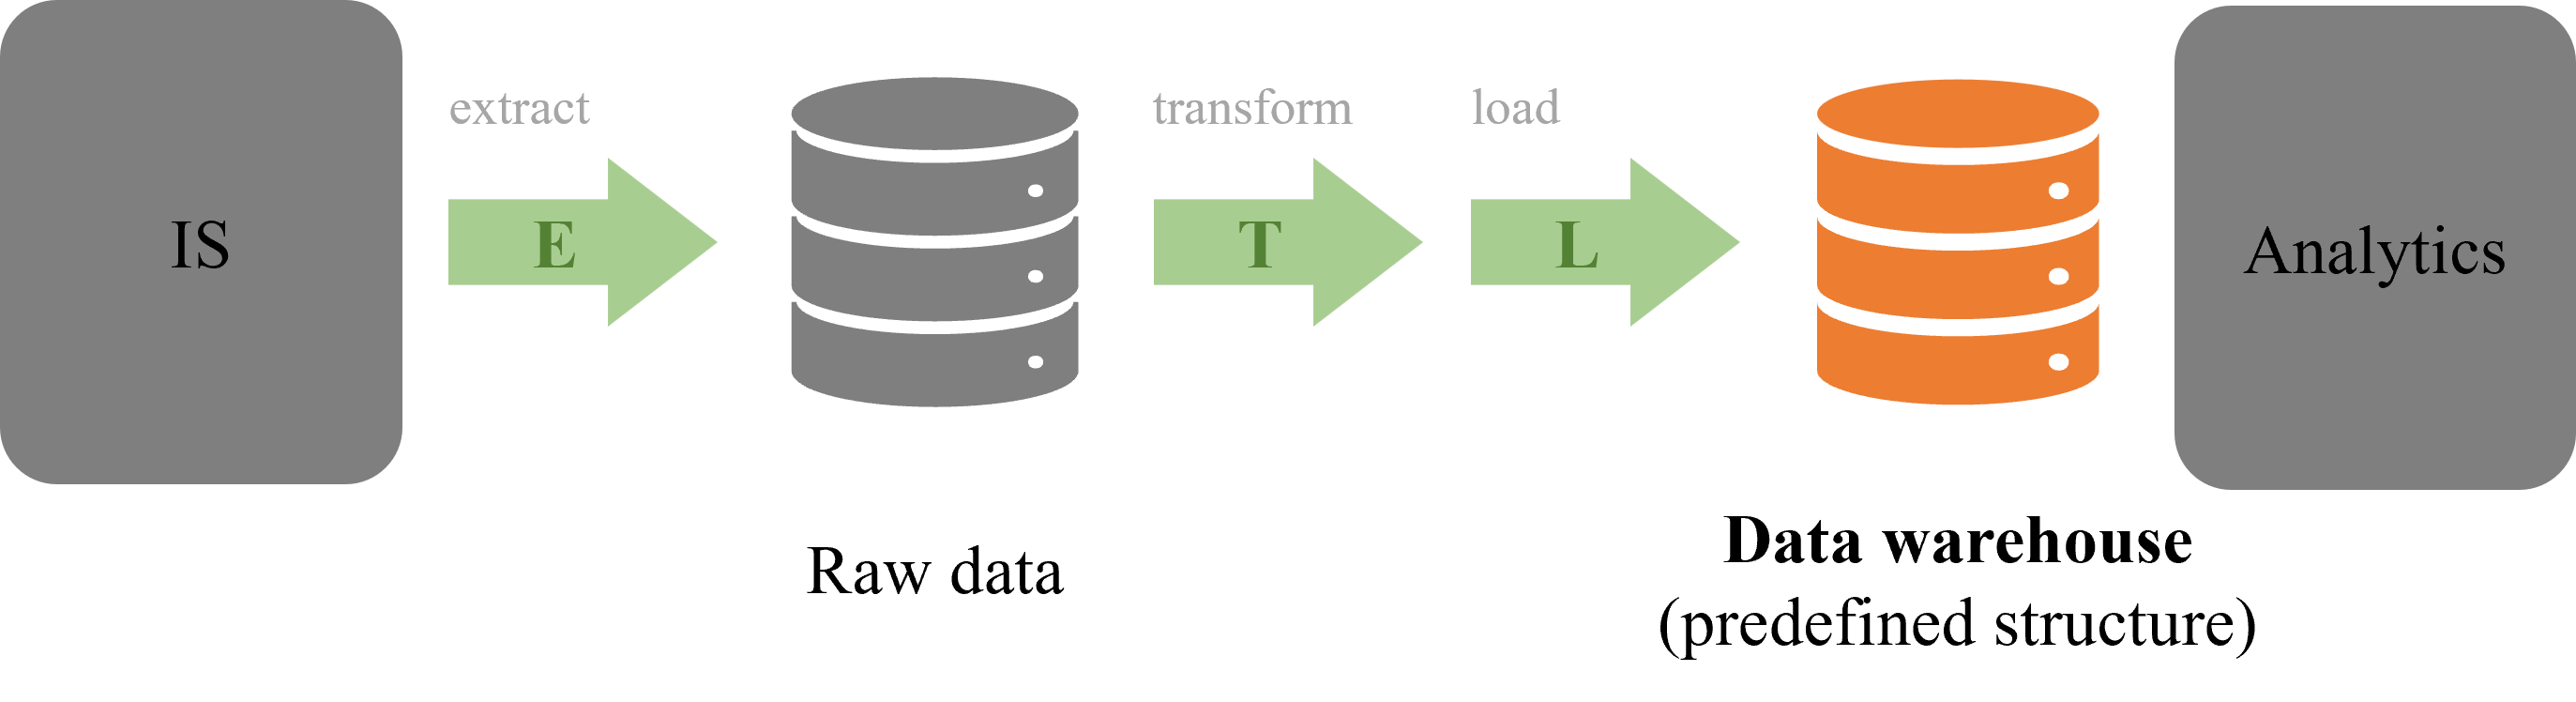
\includegraphics[width=0.45\textwidth]{assets/basics/etl.png}% TODO: adjust
  \caption{Handling outliers in box plots}
  \label{fig:2_box_plot_outlier_handling}
\end{figure}